\documentclass[12pt, a4paper, titilepage]{article}
\usepackage{graphicx}
\usepackage{subcaption}
\graphicspath{{C:/Users/huawei/Desktop/imag es/}} \usepackage{easyReview}
\usepackage{setspace}
\usepackage[english]{babel}
\usepackage[utf8x]{inputenc}
\usepackage{amsmath}
\usepackage{hyperref}
\usepackage{apacite}
\usepackage{titlesec}
\usepackage{dcolumn}
\usepackage{lscape}
\usepackage{pdflscape}
\usepackage{tabularx}
\usepackage{xcolor}
\usepackage{multirow}
\usepackage{times}
\usepackage{booktabs}
\usepackage{fancyhdr}
\usepackage[margin=1in]{geometry}
\usepackage{color}
\usepackage{dcolumn}
\usepackage{siunitx}
\usepackage{array}
\usepackage{longtable}
\usepackage{lineno}
\usepackage{array}
\usepackage{siunitx}
\usepackage{listings}
\usepackage{regexpatch}
\usepackage{multicol}
\usepackage{bm}
\usepackage{lineno}
\usepackage{color, colortbl} %righe colorate
\usepackage{lineno}
\usepackage{easyReview}
\usepackage{amssymb}

\usetikzlibrary{shapes.geometric, arrows}

\tikzstyle{startstop} = [rectangle, rounded corners, minimum width=3cm, minimum height=1cm,text centered, draw=black, fill=red!30]
\tikzstyle{process} = [rectangle, minimum width=3cm, minimum height=1cm, text centered, draw=black, fill=orange!30]
\tikzstyle{decision} = [diamond, minimum width=3cm, minimum height=1cm, text centered, draw=black, fill=green!30]
\tikzstyle{arrow} = [thick,->,>=stealth]

% formattazione per APA 7 

\raggedbottom
\titleformat*{\section}{\bfseries\centering}
\titleformat*{\subsection}{\bfseries\flushleft}
\titleformat*{\subsubsection}{\bfseries\itshape\flushleft}
\titleformat*{\paragraph}{\bfseries}
\titleformat*{\subparagraph}{\large\bfseries}


%opening
\title{The good, the bad, and the ugly}
\author{}

\begin{document}

\vspace*{10mm}
\begin{center}
	\begin{LARGE}
 New Item Response Theory based algorithms for the development of short test forms
	\end{LARGE}
	
	\vspace{5mm}
	\begin{large}
		\doublespacing
		Ottavia M. Epifania\textsuperscript{1}, Pasquale Anselmi\textsuperscript{2}, and Egidio Robusto\textsuperscript{2} \\ 	\vspace{1.5mm}
		\textsuperscript{1} Department of Psychology and Cognitive Science, University of Trento, IT \\ \vspace{1.5mm}
	\textsuperscript{2}	Department of Philosophy, Sociology, Education, and Applied Psychology, University of Padova, IT
	\end{large}
\end{center}
\vspace{15mm}
\begin{center}
	\textbf{Author Note}
\end{center}
	
	Ottavia M. Epifania 
\includegraphics[width=0.06\linewidth]{orcid.png} https://orcid.org/0000-0001-8552-568X
	
	Pasquale Anselmi 
\includegraphics[width=0.06\linewidth]{orcid.png} https://orcid.org/0000-0003-2982-7178 
	
	Egidio Robusto 
\includegraphics[width=0.06\linewidth]{orcid.png} https://orcid.org/0000-0002-7583-2587
	
	\vspace{5mm}
	The authors have no conflict of interest to disclose.
	
	\vspace{5mm}
	
	Correspondence concerning this article should be addressed to: Ottavia M. Epifania, Department of Psychology and Cognitive Science, Corso Bettini 84, Rovereto, Trento, Italy. \\
	E-Mail: ottavia.epifania@unitn.it \\



\vfill

%\end{document}

\newpage

\begin{center}
	\textbf{ New Item Response Theory-Based Algorithms for the Development of Short Test Forms}
\end{center}

\vspace{5mm}

\begin{abstract}
	\onehalfspacing
This manuscript presents Item Response Theory-based algorithms for the development of short test forms (STFs) from full-length tests. All algorithms aim at minimizing both the number of items included in the STF and the minimum average distance from a target test information target (TIF) that describes the desired characteristics of the STF, denoted as TIF-target. The algorithms differ according to the method used for including an item in the STF at each iteration, while they share the same termination criterion. 
The item selection is based on the ability of each item to reduce the distance from the TIF-target considering either one specific latent trait level defined at each iteration or the entire latent trait level.
The algorithms stop when the last selected item does not contribute in reducing the distance from the TIF-target. 
The performance of the algorithms is compared against that of a brute force algorithm, which selects the item combination best able to reduce the distance from the TIF-target among all the possible item combinations.  Results of a simulation study show that the algorithm that selects the items according to their ability of reducing the distance from the TIF-target throughout the entire latent trait outperforms the other algorithms. Limitations of the study and future lines of research are discussed.

\textbf{Keywords:} Item Response Theory; Information Functions; Algorithms; Short Test Forms
\end{abstract}


\newpage

\doublespacing


\newpage
\begin{center}
	\textbf{ New Item Response Theory-Based Algorithms for the Development of Short Test Forms}
\end{center}


%Since Item Response Theory (IRT) provides detailed information on the measurement precision of each item across different levels of the latent trait, it constitutes an ideal framework for test development \cite<e.g.,>{baker2017, van1987absolute}. Moreover, it allows for the development of tests or short test forms  (STFs) from an item bank or from an existing test, respectively.
Item Response Theory (IRT) offers detailed insights into the measurement precision of individual items across varying levels of the latent trait, making it an ideal framework for test development \cite<e.g.,>{baker2017, van1987absolute}. By leveraging its robust analytical capabilities, IRT facilitates the construction of tests designed from item banks or the derivation of short test forms (STFs) from existing assessments. This flexibility ensures that tests can be optimized for specific purposes, populations, or contexts while maintaining precision and validity.
The STFs developed from tests can be classified into two main types.
 On the one hand, there are the adaptive STFs developed within the computerized adaptive testing framework, which tailor the item administration to maximize measurement precision for each respondent \cite<e.g.,>{magis}. Therefore, the items may differ from one respondent to another. On the other hand, static STFs are composed of the same subset of items, which is chosen to maximize the measurement precision across all the respondents.   
%The information on the measurement precision of each item can be exploited for the creation of ad-hoc STFs by selecting only those items that most precisely measure specific levels of the latent trait, in line with the aim of the assessment.  
This article presents three new IRT-based algorithms for the development of STFs. 
All algorithms attempt at recreating the desired characteristics of a test, as defined through a target information function, by iteratively selecting the items that reduce as much as possible the distance between the information function of the STF and the target one. In this application, the focus is on the development of static STFs from full-length tests, although the introduced algorithms also apply to the development of static tests from item banks.
%The methods used for selecting the items at each iteration differentiate the algorithms. Specifically, they select the items according to the item's ability of reducing the distance from the TIF-target considering either a single latent trait level defined at each iteration or the entire latent trait.  



In common IRT procedures \cite<e.g.,>{chiesi, colledani2018, silvia}, the items  are selected for inclusion in the STF according to their measurement precision with respect to different levels of the latent trait that are of interest for the assessment. To pursue this aim, the information functions of all the items in the full-length test are inspected, and the items with the information functions best able to comply with the desired characteristics of the STF are selected for inclusion. 
Although this procedure offers high degrees of freedom (e.g., the number of items in the STF does not need to be specified in advance), it strongly relies on the expertise and subjectivity of the researchers, which lead to issues related to 
replicability.   
Moreover, since this procedure is not automated, it might be particularly demanding, especially if the full-length test comprises many items. 
Recently, \citeA{pauci} introduced a procedure, denoted as $\theta$-target procedure, which integrates the principles of computerized adaptive testing (i.e., tailoring the item administration to specific latent trait levels) for the development of static STFs from full-length tests, thus allowing for its automation. 
The newly introduced procedure grounds the item selection on the measurement precision of each item in the full-length test with respect to specific latent trait levels of interest, denoted as $\theta$ targets, which are defined a priori according to the aim of the assessment. 
The procedure selects an optimal item (i.e., the item that provides the highest measurement precision) for each of the identified $\theta$ targets. 
Despite being promising, the discrete definition of the $\theta$ targets raises different issues that cannot be ignored. 
Firstly, since an optimal item is selected for each of the $\theta$ targets, the actual number of $\theta$ targets determines the number of items included in the STFs. 
As such, the more the STF is meant to precisely measure larger regions of the latent trait, the larger the number of selected $\theta$ targets and the larger the number of items that need to be included in the STF. 
Moreover, the functioning of the $\theta$-target procedure strongly depends on the availability in the item bank of informative items with respect to the defined $\theta$ targets. If the item bank does not contain informative items with respect to one or more $\theta$ targets, sub-optimal items might be included in the final item selection. As such, the STF might contain more items than actually needed or items that might not appropriately assess the levels of interest. 
Finally,  the $\theta$ targets are defined as discrete values to recreate a sort of ``overall'' information function of the STF, which is continuous by nature. 
%The $\theta_{target}$s are defined a priori according to the specific aim with which the STF is developed. For instance, if the aim of the STF is to discriminate respondents below and above a certain cut-off (e.g., clinical diagnostic tests) the $\theta$s are defined around the cut-off point, such that only the most informative items for that region of the latent trait are included in the STF. Otherwise, if the aim is to maximize the information across the entire latent trait, the $\theta_{target}$s can be equally spread along the latent trait continuum.   
%Typically, the development of STF relies on the expertise of the researchers, in that that the items are manually chosen according to the measurement precision that they provide to address the final measurement precision one wants to obtain for the STF. While such a procedure provides large degrees of freedom in terms of item selection and does not require the definition of the number of items a priori, it strongly relies on the expertise of the researcher and might be at risk of not being reproducible. 
%While both types of STFs are based on the same principle, they differ in their focus. Adaptive STFs adjust to the individual respondent’s characteristics, maximizing measurement precision for that specific person. In contrast, static STFs aim to achieve overall precision across the entire group of respondents. Both approaches leverage the information from IRT models regarding the measurement precision of each item at various levels of the latent trait.
In this light, it might be more convenient to directly refer to a continuous function describing the desired characteristics of the STF by means of a target information function to be recreated with the final selection of items in the STF \cite<e.g.,>{lordTif}.
The specification of a TIF-target allows for shifting the focus on different regions of the latent trait, hence STFs addressing different aims can be developed. 
\begin{figure}
	\centering
	\begin{subfigure}{0.45\linewidth}
		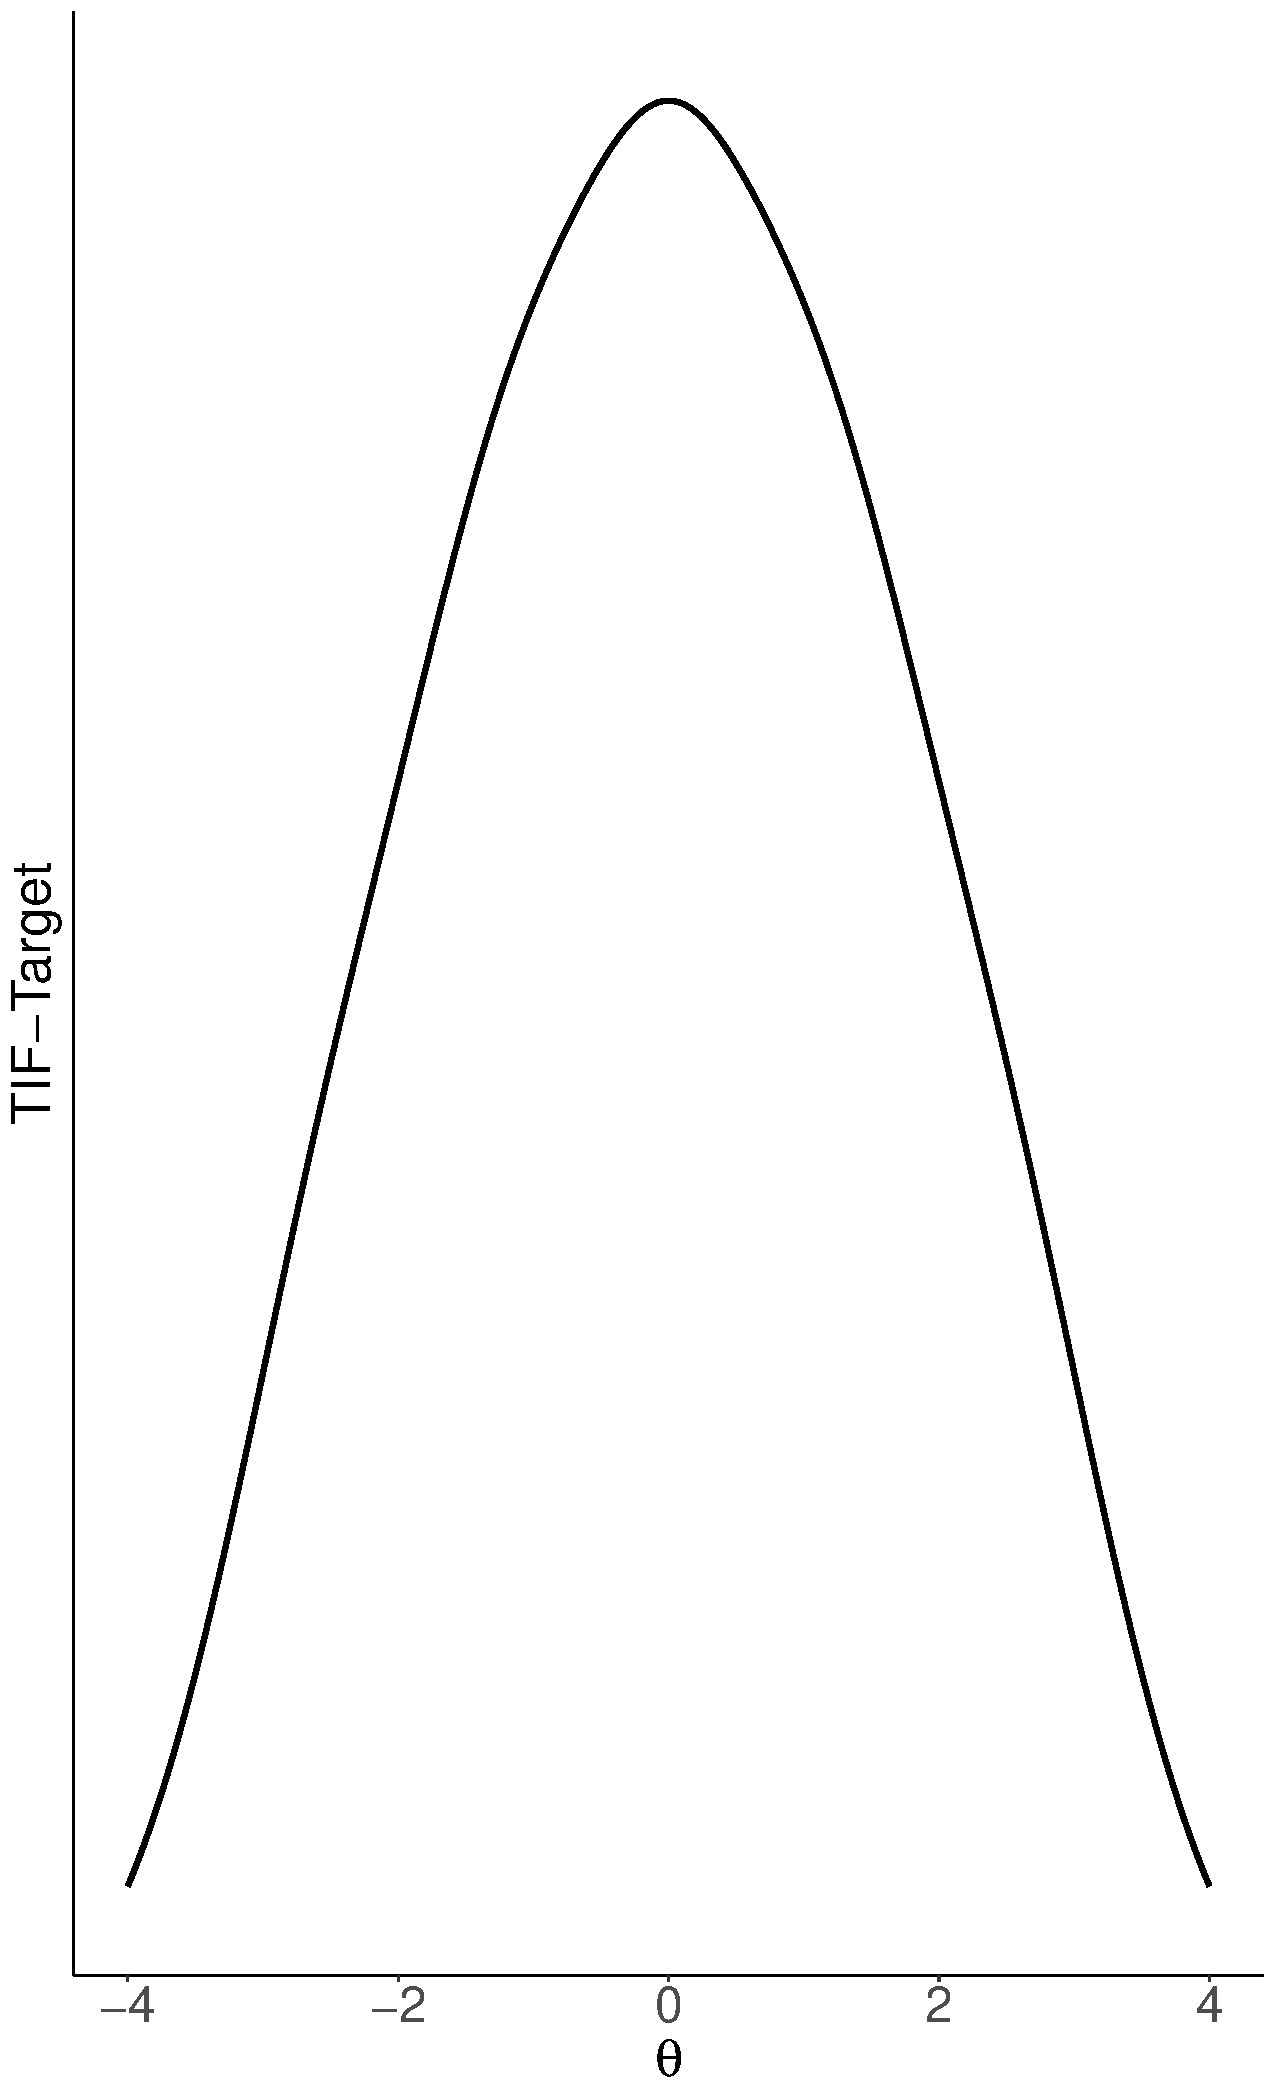
\includegraphics[width=\textwidth]{img/target_n}
		\caption{}
		\label{fig:targetN}
	\end{subfigure}
	\begin{subfigure}{0.45\linewidth}
		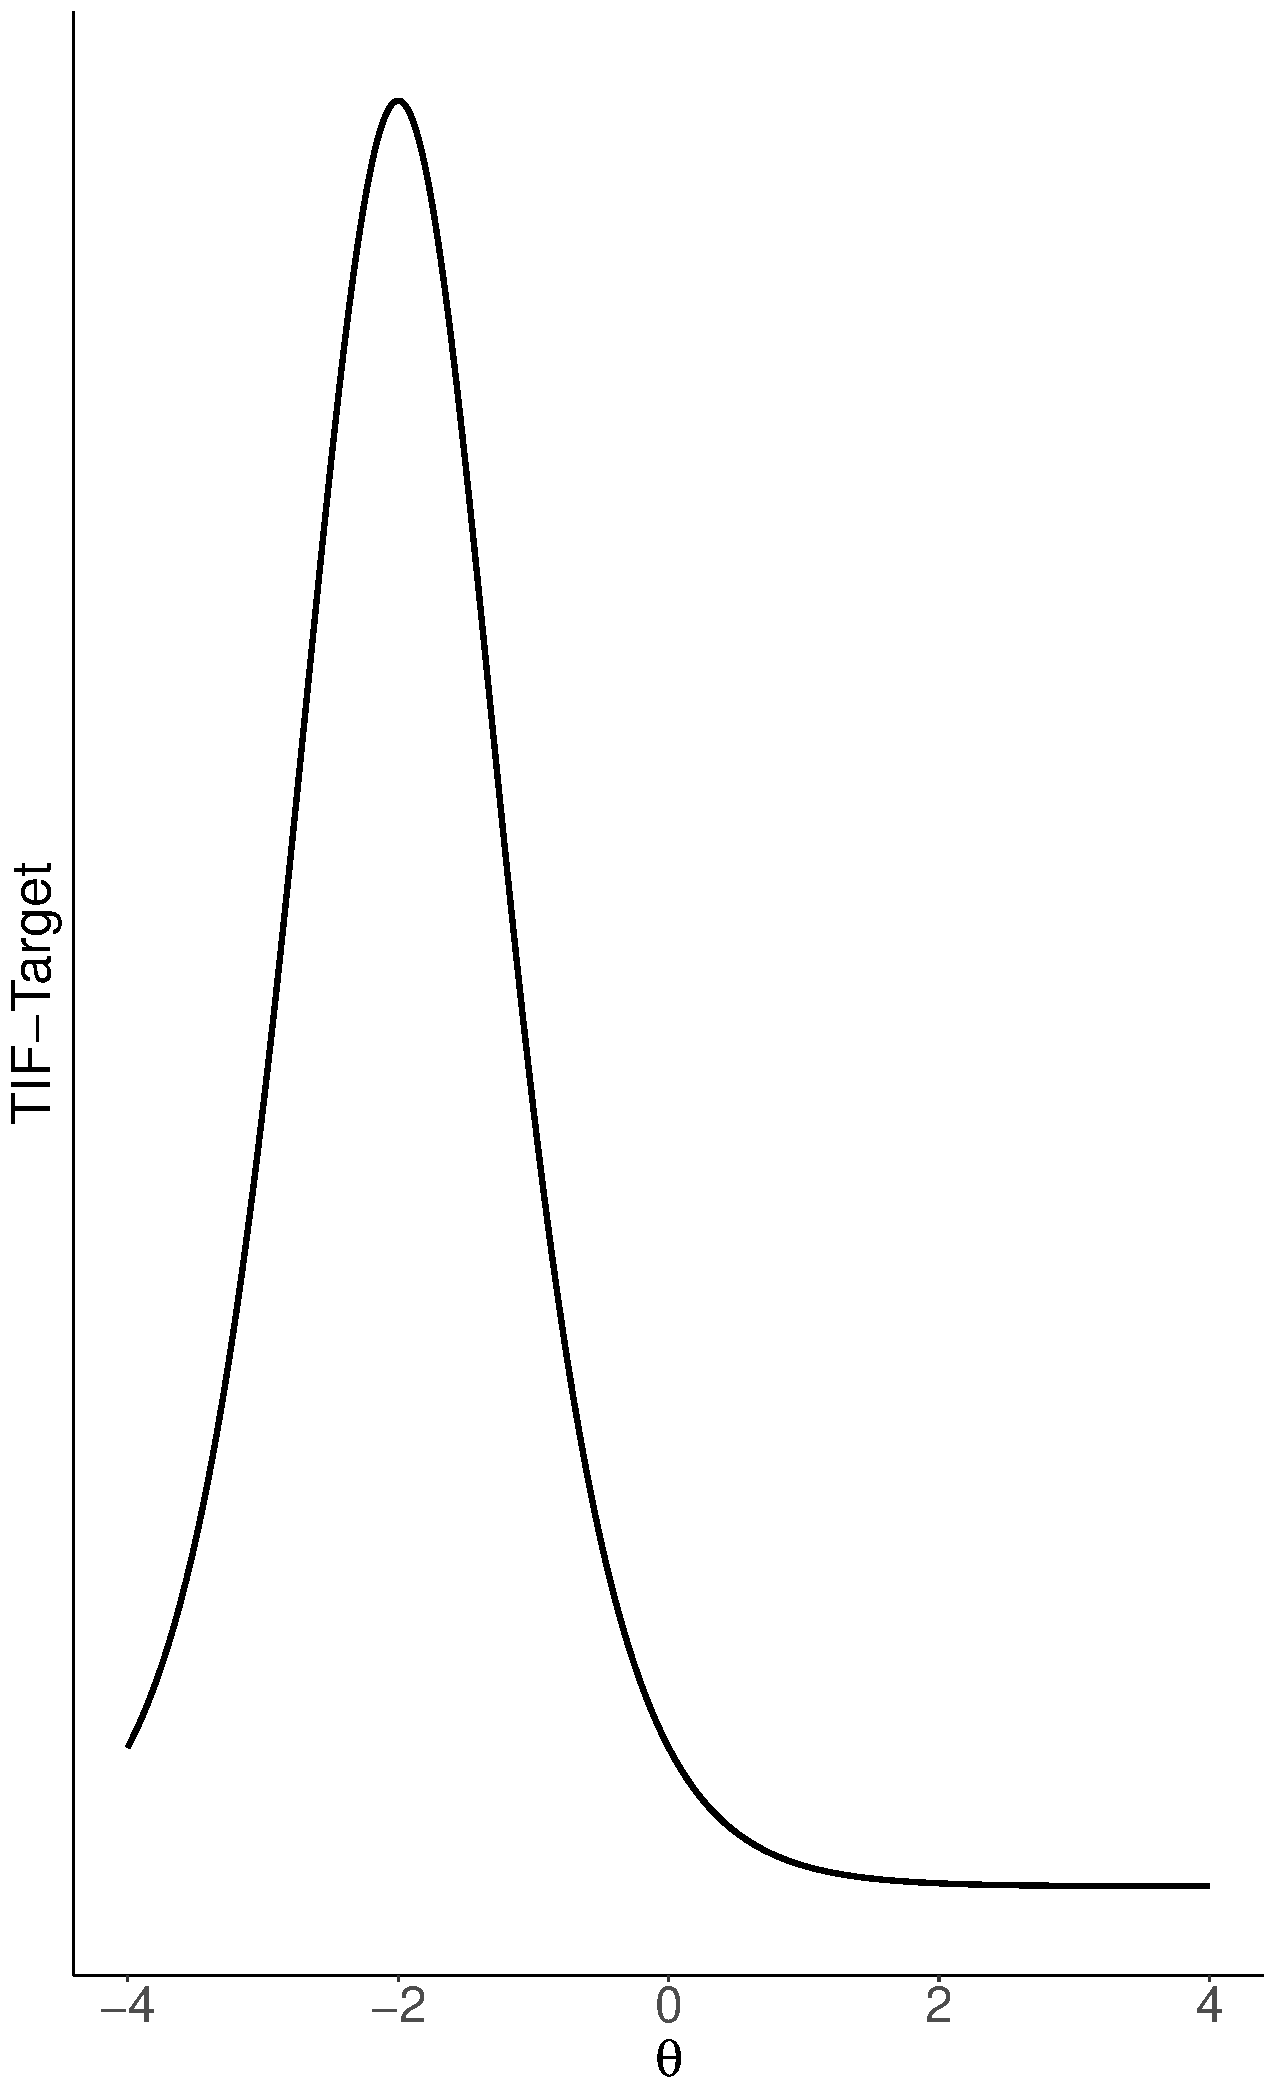
\includegraphics[width=\textwidth]{img/target_sk}
		\caption{}
		\label{fig:targetSK}
	\end{subfigure}
\caption{Examples of target information functions. Panel \ref{fig:targetN} illustrates a target information function aimed at obtaining a good measurement precision of latent trait levels between $-2$ and $2$. Panel \ref{fig:targetSK} illustrates a target information function focused on a specific level of the latent trait, $\theta = -2$.}
	\label{fig:tartge-examples}
\end{figure}
For instance, Figure \ref{fig:tartge-examples} illustrates two TIF-targets, which have been specified for obtaining either  precise measurements of different levels of the latent trait. 
Figure \ref{fig:targetN} illustrates a TIF target for obtaining a precise measurement of the $\theta$ levels between $-2$ and $2$. Figure \ref{fig:targetSK} illustrates a TIF target highly informative for $\theta$ levels around $-2$ standard deviation below the average population mean of 0 \cite<a cut off at 2 standard deviations below the population mean is a criterion sometimes used in diagnostic tests, see e.g., >{balboni, tasse2016}. 
%Specifically, Figure \ref{fig:targetN} depicts the TIF-target that allows for obtaining precise measurements across almost the entire latent trait, with a particular focus on the regions between $-2$ and $2$. Such a TIF-target might be employed when developing STFs for the assessment of psychological constructs that are normally distributed among the general population (e.g., intelligence). On the other hand, Figure \ref{fig:targetSK} depicts a TIF-target that is consistent for the development of a diagnostic STF, since its focus is on a specific $\theta$ level

\normalcolor
Although the specification of the desired characteristics of the STF through a target information function is reasonable, its actual definition might not be straightforward. While there might be an idea concerning the shape of the target information function (i.e., the regions of the latent trait on which the highest measurement precision is desired), the definition of its height (i.e., the amount of information for different levels of the latent trait) might be troublesome \cite{van1989relative}. 
In this sense, if both the shape and height of the target information function can be defined, the test or STF development is performed with the idea of recreating an \emph{absolute information} \cite{stocking, van1987absolute}. 
Conversely, if only the shape of the target information function is known and can be defined, the test or STF development is performed with the idea of recreating the shape of a \emph{relative information} \cite{van1989relative}. 

%\subsection{Existing Procedures}



%Adaptive STFs are . According to this procedure, the administration of each item depends on the responses registered at the previous items. 
%At each iteration, a temporary estimate of the latent trait level of the respondent is computed based on the responses registered up to that point, and the next administered item is the one that can maximize the information for that level.
%As such, each respondent can be administered with a different subset of items, which aims at maximizing the measurement precision for each respondent. 

%The latent trait levels on which the static STFs focus the most might change and should be defined in advance. For instance, if the STF is aimed ad the assessment of clinical population with medium-low latent trait levels, the items composing the STF should be mostly located in those regions. The STF may not be optimal in terms of maximizing measurement precision for each individual respondent. However, it would still ensure adequate measurement precision for respondents within those specific latent trait levels, providing reliable measurement for those groups.

%Although adaptive STFs are undoubtedly convenient since they allow for obtaining precise estimates of the latent trait level of each respondent by tailoring the item administration, they might be problematic in some contexts. For instance, they require the implementation of adaptive algorithms on ad-hoc platforms for the administration, which might not be always accessible or they might be difficult to use with some target populations (e.g., the elderly). Moreover, fairness issues might be raised in evaluation contexts where it is important to administered all respondents with the same subset of items.  
 

This manuscript presents three new IRT-based algorithms for the development of STFs, which ground the item selection on the definition of the general desired characteristics of the STF as expressed by a target test information function. The continuous definition of the desired characteristics allows for overcoming the issues related to the a priori specification of $\theta$ targets, hence releasing the constraint on the optimal number of items. As the  target information function is empirically defined with a specific shape and height, these algorithms attempt at finding the item selection to include in the STF that is best able to reduce the distance from an absolute information.
All algorithms consider the distance between the target information function and the information function obtained on the items selected up to that iteration with the aim of bridging the gap between the two information functions (i.e., bringing the information function of the STF as close as possible to the target one). As it will be further illustrated, they differ according to how they consider the distance between the information functions and hence on how they consider the items for inclusion in the STF. The performance of the algorithms is evaluated in a simulation study, where it is compared against that of a brute force algorithm. 
Since the brute force algorithm selects the item combination best able to reduce the distance from the target information function among all the possible item combinations of different length, its item selection is considered as the gold standard. 




\normalcolor

% This contribution is focused on the development of STFs from full-length tests. Nonetheless, the presented algorithms can be also used for the development of informative tests developed from item banks.


The manuscript is organized as follows. The next section illustrates the IRT model used as reference in this work, along with the definition of the related information functions. The proposed algorithms are then presented, followed by a simulation study that compares their performance in STFs development. The manuscript concludes with final remarks.

%Come limitazione il fatto che il numero dei theta target influenza molto il numero di item da inserire, tanto che più theta target ci sono più item devono essere includi nella forma breve ma forse più importante il fatto che è basata su valori puntuali del tratto latente quando forse sarebbe più comodo definer una tif generale da riprodurre (riprendere il discorso di Tif relativa e Tif assoluta e dire chiaramente che in questo caso ci muoviamo nel caso di una tif assoluta visto che viene definita un'altezza dell'infromazione ma che in futuro ci contreeremo sulla tif relativa)



\section*{Item Response Theory and Information Functions}
Different IRT models are available for the analysis of dichotomous responses, which differentiate according to the characteristics of the items that they take into account. 
In this application, 
the 2-Parameter Logistic model \cite<2-PL;>{birnbaum1968} is used as a reference, which considers item difficulty and item discrimination. However, the presented approach can be applied to other IRT models that consider item discrimination. According to the 2-PL model, the probability of observing a positive response by person $p$ on item $i$ is formalized as: 

\begin{equation}
	P(x_{pi} = 1|\theta_p, b_i, a_i) = \dfrac{\exp [a_i(\theta_p - b_i)]}{1 + \exp [a_i(\theta_p - b_i)]},
\end{equation}
where $\theta_p$ is the ability parameter of person $p$ (i.e., the latent trait level of $p$), $b_i$ is the difficulty parameter of item $i$ (i.e., the location of $i$ on the latent trait), and $a_i$ is the discrimination parameter of item $i$ (i.e., the ability of $i$ to distinguish between respondents with different levels of $\theta$). The probability of observing a positive response changes as the distance between the ability of the person $\theta_p$ and the location of the item on the latent trait $b_i$ changes. This probability is .50 when the ability of person $p$ matches the difficulty of item $i$.

Let $B$ denote the set of items in a test or in an item bank. The precision with which each item $i \in B$ measures different levels of the latent trait is described by the \emph{item information function}, $\text{IIF}_i = a_i^2P(x_{pi} = 1|\theta, b_i, a_i)[1- P(x_{pi} = 1|\theta, b_i, a_i)]$. In the 2-PL model, the IIF reaches its maximum when $\theta_p = b_i$. The precision with which the test as a whole measures the entire latent trait is expressed by the \emph{test information function}, which is the sum of the IIFs of all the items in a test or item bank, $\text{TIF} = \sum_{i \in B} \text{IIF}_i$. 
The shape and height of the TIF depends on the spread of the items along the latent
trait continuum and on their discriminability.
 Since the TIF is the sum of the IIFs, the higher the number of items in the test, the higher the TIF. Alternatively, a mean TIF can be computed by averaging for the number of items. As it will be further illustrated, the computation of the mean TIF might be more convenient when developing STFs.


\normalcolor

\section*{The Algorithms}

The three introduced algorithms aim at approximating as best as possible the desired characteristics of a test, as expressed by a target information function (TIF-target), by selecting the items best able to reduce the distance between the information function of the provisional STF (pSTF) and the target one. 
Two of the algorithms (denoted as item locating algorithm -- ILA -- and item selecting algorithm -- ISA --) can be seen as the natural evolution of the $\theta$-target procedure in that they ground the item selection on the characteristics of each item with respect to a specific $\theta$ target, which is defined at each iteration as the latent trait level where the distance between the two information functions is maximum.
The third one (Frank) overcomes the definition of the $\theta$ targets altogether by considering the entire latent trait for the item inclusion at each iteration. As such, it accounts for the measurement precision of each item with respect to the entire latent trait and to the TIF-target. 
All three algorithms attempt at bridging the gap between the TIF-target and the temporary information function obtained from the items selected up to that iteration. 
By grounding the item selection on a specific $\theta$ target, ILA and ISA bring the two information functions closer considering only one latent trait level at the time. 
On the other hand, by grounding the item selection on the contribution of each item to the temporary information function, Frank bridges the gap between the two functions considering the entire latent trait. 
%However, ILA and ISA attempt at bridging the gap between the two information functions considering one discrete level at the time, the $\theta$ target, while Frank considers the entire latent trait. 
%As such, ILA and ISA select the best item according to one specific point of the latent trait, while Frank  selects the item that allows for bridging the gap between the information functions throughout the entire latent trait. 
%\color{red} Forse questa parte si può togliere 
%In ILA and ISA, the $\theta$ targets are defined at each iteration as the level of the latent trait for which the maximum distance between the information function obtained from the items selected up to that iteration and the target information function is observed. 
%Differently from the $\theta$-target procedure, the number of items does not need to be defined a priori and the algorithms automatically searches for the levels of the latent trait that need to be addressed at each iteration. The main issue of ILA and ISA pertains the items selection grounded on discrete levels of the latent trait, instead of considering its continuous nature. 
%Frank aims at overcoming this issue by considering the continuous nature of the target information function. At each iteration, it explores the distance between the target information function and the information function obtained with the items selected up to that iteration, and selects the item that is best able to bridge the gap between the target and the temporary information function considering the entire latent trait. 
\normalcolor

The ability of ILA, ISA, and Frank to approximate an absolute TIF-target is evaluated by comparing their performance against that of a brute force algorithm.
This algorithm
 tries every possible combination of items without repetition and selects the one best able to bridge the gap between the two information functions among all the possible item combinations attainable from the full-length test. As such, its resulting STF is considered as the gold standard.


All algorithms but the brute force start with an empty item collection, $Q$, in which an item is included at each iteration until the termination criterion is met.  %Since each algorithm starts with an empty set and adds one item at each iteration, the mean TIF is computed at each iteration by considering the number of items in the current set $Q$.
Before any item can be included in $Q$, the termination criterion tests its usefulness in reducing the distance from the TIF-target by concurrently considering the TIF-target, the TIF obtained from the STF with the last item considered for inclusion (i.e., provisional item), and the TIF obtained from the STF without this last item. 
%At each iteration, the termination criterion tests whether other items should be added in the STF by considering the distance between the TIF-target, the TIF obtained by adding the last item considered for inclusion (i.e., provisional item), and the TIF obtained without this item. 
If the distance between the former two is greater than or equal to the distance between the latter two, the provisional item is not included in the STF and the algorithm stops. Vice versa, the item is included and the algorithms proceeds to a new iteration. The reasoning is as follows. If the distance between the TIF-target and the STF including the provisional item is greater than or equal to the difference between the TIF-target and the STF without the provisional item, the provisional item does not contribute in reducing this distance. 
Since the provisional item is the best one among the available options according to the selection method of each algorithm and does not contribute to reduce the distance from the TIF-target, the algorithm stops. 
When the termination criterion is reached, the final item selection included in the STF is the one in $Q$ up to the last iteration, which does not include the provisional item.

In what follows, the notation $||X||$ is used to denote the cardinality of a generic set $X$, $B$ denotes the set of items in the full-length test, $Q_x$ indicates the subset $Q_x \subset B$ of items included in the STF by each algorithm $x \in \{\text{Bruto}, \text{ILA}, \text{ISA}, \text{Frank}\}$, and $\text{TIF}^*$ indicates the TIF-target. The TIF-target is used to express the desired characteristics of the STF in terms of absolute information across the latent trait. 
Since the focus of the manuscript is on the development of STFs from full-length tests, $Q_x$ is taken to be a proper subset of the items in the test, such that it is not possible to obtain a STF that contains all the items of the test. If the algorithms are applied for the generation of informative tests from an item bank, $Q_x$ can be the subset of $B$, and all the items can be included in the test. 

 
%\add{current number of items in the STF, va ben definito da qualche parte. nei cofnronit si parla di una stf che è in divenire a partire  da un insieme vuoto di item e che la media è calcolata sulla base del numero di item che sono presenti in quel momento anella STF}

The brute force algorithm (i.e., Bruto) does not have a proper termination criterion given that it generates all the possible STFs of different length and then chooses the one that allows for minimizing the distance from the $\text{TIF}^*$. It follows that Bruto does not have iterations either. 
%For all other algorithms, the termination criterion is the same. 
%Specifically, it tests whether the last provisional item (i.e., the item that is being evaluated for the inclusion in the STF at the current iteration) is useful in reducing the distance from the $\text{TIF}^*$. 
%If the distance between the $\text{TIF}^*$ and the provisional TIF that includes the last provisional item (denoted as $\text{pTIF}$) is greater than or equal to the distance between the $\text{TIF}^*$ and the TIF obtained without the provisional item, this is deemed as not useful in reducing the distance from the $\text{TIF}^*$ and the algorithm stops.  The subset of items would hence be the one at the previous iteration, excluding the provisional item. 
%If the same comparison is false, the provisional item is deemed as useful in reducing the distance from the $\text{TIF}^*$, it is included in the subset of items and a new iteration starts. 
%Not having a termination criterion, Bruto does not have iterations either. Indeed, Bruto generates all the possible STFs of different lengths considering different combination of items, and it chooses the one that is best able to reduce the distance from the $\text{TIF}^*$.
%Bruto is the only algorithm for which the number of iterations is known in advance, since it compares the TIF attainable from all the possible combinations of items of different length from an item bank \add{non so se sia corretto parlare di number of iterations}. 
The number of iterations performed by the other algorithms cannot be known in advance since they iteratively compare the TIF obtained by including the provisional item with the $\text{TIF}^*$ until the termination criterion is met. 
The only constraints on the number of iterations pertains the lower and upper bound. 
 Specifically, since all the algorithms start from an empty set of items, they are forced to perform at least two iterations such that at least one item can be included in the STF. Moreover, the upper constraint is logically imposed by the number of items in the full-length test, such that the maximum number of iterations is equal to the cardinality of the full-length test. Importantly, if the algorithms reach the last iteration and the termination criterion is not met, it is considered as a failure in the their ability to find a STF able to reproduce the $\text{TIF}^*$.

 Finally, since the TIF is usually obtained by summing the IIFs together, the more the items in a test, the higher the TIF. 
 As such, when the TIF is used as criterion for deciding the best subset of items to include in a STF, the risk is to favor STFs that include more items. 
 To avoid this risk, the mean TIF of the STF is used in the comparison against the TIF-target. In what follows, the mean  TIF is simply indicated as TIF. 

 
 

\subsection*{Bruto}


Bruto compares the TIF of all the possible item combinations attainable from the items in $B$ against the $\text{TIF}^*$ and selects the item combination best able to reduce the average distance from the $\text{TIF}^*$, as follows:  

%\begin{tikzpicture}[node distance=2cm]
%	
%	% Nodes
%	\node (start) [startstop] {Start: $\forall Q \in\mathcal{Q} = 2^B \setminus \{\emptyset, B\}$};
%	\node (step1) [process, below of=start] {Step 1: Compute $\mathbf{TIF}^Q = \frac{\sum_{i \in Q} IIF_i}{||Q||}$};
%	\node (step2) [process, below of=step1] {Step 2: Compute $\overline{\Delta}_{\mathbf{TIF}^Q} = \mathit{mean}(|\mathbf{TIF}^* - \mathbf{TIF}^Q|)$};
%	\node (end) [startstop, below of=step2] {End: $Q_{bruto} = \arg \min_{Q \in \mathcal{Q}} \overline{\Delta}_{\mathbf{TIF}^Q}$};
%	
%	% Arrows
%	\draw [arrow] (start) -- (step1);
%	\draw [arrow] (step1) -- (step2);
%	\draw [arrow] (step2) -- (end);
%	
%\end{tikzpicture}

$\forall Q \in\mathcal{Q} = 2^B \setminus \{\emptyset, B\}$, compute

\begin{enumerate}
	\item $TIF^{Q} =  \frac{\sum_{i \in Q} IIF_i}{||Q||}$ and
	\item $\overline{\Delta}_{\text{TIF}^{Q}} =  \mathit{mean}(|TIF^* - TIF^{Q}|)$. 
\end{enumerate}


Then, $Q_{bruto} = \arg \min_{Q \in \mathcal{Q}} \overline{\Delta}_{\mathbf{TIF}^{Q}}$.

For all the possible item combinations in $\mathcal{Q}$ that are attainable from the item bank $B$ (excluding the empty set and the full set of items), Bruto computes: (1.) the mean TIF, $TIF^Q$ and (2.) 
the average distance $\overline{\Delta}_{\text{TIF}^Q}$ between the $\text{TIF}^*$ and the $\text{TIF}^Q$.  Then, the final subset of items of the STF, $Q_{bruto}$, is the one that allows for obtaining the least value of $\overline{\Delta}_{\text{TIF}^{Q}}$, hence for minimizing the distance from the $\text{TIF}^*$.

Given that Bruto attempts all the possible item combinations in $\mathcal{Q}$, it ensures to find the one that is best able to minimize the average distance from the $\text{TIF}^*$.
% that aims at the selection of best combination of items to recreate a given $TIF^*$  by comparing the TIF-target with the TIF obtained with all the possible combinations of items of different lengths that are obtainable from an item bank $B$. The total number of item combinations of different lengths $\mathcal{Q}$ is equal to the power set of the item bank minus the empty set and the full set of items. For each item combination $Q \in \mathcal{Q}$, the mean TIF $TIF^Q$ is computed, and is compared against the TIF-target. Specifically, the average distance between the TIF-target and $TIF^Q$ is computed and the item combination selected by Bruto is the one among all item combinations that allows fro minimizing the distance between $TIF^*$ and $TIF^Q$.

\subsection*{Item Locating Algorithm}


At each iteration $k$, the item locating algorithm (ILA) selects the item that minimizes the distance on the latent trait from a specific $\theta$ target (denoted as $\theta_{target}$), as follows:


At $k = 0$: $\text{TIF}^0(\theta) = 0 \, \forall \theta$, $Q^0 = \emptyset$. For $k \geq 0$,
\begin{enumerate}
	\item $\theta_{target} := \arg \max |\text{TIF}^* - \text{TIF}^{k}|$
	\item $i^* := \arg \min_{i \in B\setminus Q^{k}} |\theta_{target} - b_i|$
	\item $\text{pTIF}_{i^*} = \frac{TIF^k + IIF_{i^*}}{||Q^{k}|| + 1}$ %$\mathbf{pTIF}_{i^*}= \frac{\sum_{i \in Q^{k} \cup \{i^*\}} IIF_i}{||Q^{k} \cup \{i^*\}||}$ $=$ 
	\item Termination Criterion: $|\text{TIF}^* - \text{pTIF}_{i^*}| \geq |\text{TIF}^* - \text{TIF}^{k}|$: 
	\begin{itemize}
		\item FALSE:  $Q^{k+1} = Q^{k} \cup \{i^*\}$, $\text{TIF}^{k+1} = \text{pTIF}_{i^*}$, iterates 1-4 
		\item TRUE: Stop, %The item in $i^*$ does not contribute to reduce the distance from the TIF-target, hence: 
		$Q_{ILA} = Q^k$
	\end{itemize}
\end{enumerate}

ILA starts at iteration $k=0$, where $Q^0 = \emptyset$ and $\text{TIF}^0(\theta)$ is 0 for all the values of $\theta$. 
At each iteration: (1.) the $\theta_{target}$ is defined as the latent trait level for which the highest distance between the $\text{TIF}^*$ and the $\text{TIF}^k$ is observed; (2.) The item $i \in B\setminus Q^k$ for which the minimum distance from the $\theta_{target}$ is observed is considered as the provisional item $i^*$; (3.) A provisional TIF, $\text{pTIF}_{i^*}$ is computed as the average TIF considering the items in $Q^k$ and item $i^*$, with the condition $i \in B\setminus Q^k$ ensuring that the items are selected only once; and (4.)
The termination criterion tests whether the provisional item $i^*$ is useful for reducing the distance from the $\text{TIF}^*$. Specifically, if the distance between the $\text{TIF}^*$ and the $\text{pTIF}_{i^*}$ (TRUE) is greater than or equal to the distance between the $\text{TIF}^*$ and the $\text{TIF}^k$ (i.e., the TIF obtained by considering the item in $Q^k$, without item $i^*$), the item in $i^*$ does not help in reducing the distance from the $\text{TIF}^*$. As such, ILA stops, and  the subset of items selected by ILA, $Q_{ILA}$, is the one in $Q^k$. 
Conversely (FALSE), if the distance between the $\text{TIF}^*$ and the $\text{pTIF}_{i^*}$ is lower than that between the $\text{TIF}^*$ and the $\text{TIF}^k$, then the item in $i^*$ is useful in reducing the distance from the TIF-target, it is included in the set of selected items, and a new iteration starts, $Q^{k+1} = Q^k \cup \{i^*\}$

%In this sense, ILA is based on the distances between the locations of the items on the latent trait (the difficulty parameter $b_i$) and the $\theta_{target}$. 
%The $\theta_{target}$ corresponds to the level of the latent trait for which the maximum distance between the $TIF^*$ and the TIF containing the subset of items selected up to that the iteration, $Q^k \subset B$, is observed.  
%The termination criterion tests whether the average distance between the $TIF^*$ and the provisional TIF obtained including the last selected item $i^*$ (denoted as $pTIF_{i^*}$) is greater than or equal to the distance between the $TIF^*$ and the TIF obtained from the items in $Q^k$. If this is true, it means that the last selected item $i^*$ does not help in reducing the distance from the $TIF^*$, hence ILA stops and the final set of items is the one without item $i^*$, such that $Q_{ILA} = Q^k$. 
%Otherwise, if the termination criterion is not met, the last selected item is included in the set $Q$, such that $Q^{k+1} = Q^k \cup \{i^*\}$, and a new iteration starts. 


\subsection*{Item Selecting Algorithm}

The item selecting algorithm (ISA) follows the same procedure as ILA. However, ILA and ISA differentiate according to the method with which the provisional items $i^*$ are considered for inclusion at each iteration. While ILA selects the item that minimizes the distance on the latent trait from the $\theta_{target}$, ISA selects the item that maximizes the IIF with respect to the $\theta_{target}$, as follows: 

At $k = 0$: $\text{TIF}^0(\theta) = 0 \, \forall \theta$, $Q^0 = \emptyset$. For $k \geq 0$,

\begin{enumerate}
	\item $\theta_{target} := \arg \max |\text{TIF}^* - \text{TIF}^{k}|$
%	\item $IIF_{i \in B \setminus Q^k}(\theta_{target}) = a_i^2P(\theta_{target}, a_i, b_i)[1-P(\theta_{target}, a_i, b_i)]$
	\item $i^* := \arg \max_{i \in B\setminus Q^k} \text{IIF}_i(\theta_{target})$
	\item $\text{pTIF}_{i^*} = \frac{TIF^k + \text{IIF}_{i^*}}{||Q^{k}|| + 1}$
	\item Termination Criterion: $|\text{TIF}^* - \text{pTIF}_{i^*}| \geq |\text{TIF}^* - \mathbf{TIF}^{k}|$: 
	\begin{itemize}
		\item FALSE:  $Q^{k+1} = Q^{k} \cup \{i^*\}$, $\text{TIF}^{k+1} = \text{pTIF}_{i^*}$, iterates 1-4 
\item TRUE: Stop, %The item in $i^*$ does not contribute to reduce the distance from the TIF-target, hence: 
$Q_{ISA} = Q^k$
	\end{itemize}
\end{enumerate}
Since the procedure is the same as that described for ILA, it will not be discussed further. The only difference concerns the second step of the algorithm (2.), that is the inclusion of the items $i \in B \setminus Q^k$ in $\{i^*\}$. At each iteration, the provisional item $i^*$ that is considered for inclusion in $Q^k$ is the one that maximizes the IIF for the specific $\theta_{target}$.



\subsection*{Frank}

Instead of grounding the item selection at each iteration on a single latent trait level (i.e., the $\theta_{target}$) as ILA and ISA do, Frank considers the entire latent trait for the item selection, in that it selects the item whose IIF is best able to reduce the distance from the $\text{TIF}^*$ along the entire latent trait, as follows:

 
At $k = 0$: $\text{TIF}^0(\theta) = 0 \, \forall \theta$, $Q^0 = \emptyset$. For $k \geq 0$,

\begin{enumerate}
	\item  $A^k = B \setminus Q^k$ 
	\item $\forall i \in A^k$, $pTIF_{i}^k = \frac{\text{TIF}^k + \text{IIF}_{i}}{||Q^k||+1}$
	\item $i^* = \arg \min_{i \in A^k} |\text{TIF}^* - \text{pTIF}_i|$
	\item Termination criterion: $|\text{TIF}^* - \text{pTIF}_{i^*}| \geq |\text{TIF}^* - \text{TIF}^{k}|$: 
	\begin{itemize}
		\item FALSE:  $Q^{k+1} = Q^{k} \cup \{i^*\}$, $TIF^{k+1} = pTIF_{i^*}$, iterates 1-4 
\item TRUE: Stop, %The item in $i^*$ does not contribute to reduce the distance from the TIF-target, hence: 
$Q_{Frank} = Q^k$
		
	\end{itemize}
\end{enumerate}

When Frank starts ($k = 0$), the subset of items $Q^0$ is empty and the $\text{TIF}^0$ is 0 for all the $\theta$ levels. 
At each iteration $k$: (1.) a set of available items is generated as the items in the item bank that have not been included in the STF yet, $A^k = B \setminus Q^k$; (2.)
An average provisional TIF, $\text{pTIF}$, is computed by adding the IIF of each of the items in the set of the available items $A^k$, one at the time, to the TIF obtained from the items in $Q^k$ (The denominator is obtained by adding 1 to the cardinality of $Q^k$); (3.) Among all the items in $A^k$, the one that allows for minimizing the distance between $\text{pTIF}$ and $\text{TIF}^*$ is included in $i^*$; (4.) 
The termination criterion is tested. 
If the distance between the $\text{TIF}^*$ and the $\text{pTIF}_{i^*}$ is greater than or equal to the distance between the $\text{TIF}^*$ and the $\text{TIF}^k$ (i.e., the TIF obtained from the items in the subset $Q^k$, without item $i^*$) (TRUE), then the item $i^*$ does not contribute in the reduction of the distance from the $\text{TIF}^*$, the algorithm stops, and the final item selection is the one without the item in $i^*$, $Q_{frank} = Q^k$. Conversely (FALSE), the item in $i^*$ does contribute in the reduction of the distance from the $\text{TIF}^*$, hence it is included in the set of items and a new iteration starts, $Q^{k+1} = Q^k \cup \{i^*\}$.

%Specifically, at each iteration $k$ a set of available items is created as the items that are in the item bank and that have not been selected for inclusion in the STF yet, $A^k = B \setminus Q^k$. Then, for every item in $A^k$, a $pTIF$ is computed by adding the IIF
%of each item (one at a time) to the $TIF$ obtained from the items in $Q^k$ (i.e., the subset of items selected up to that iteration). The item whose IIF allows for reducing the distance from the $TIF^*$ is included in $i^*$ and the termination criterion (the same as that for ILA and ISA) is checked. If the average distance between the $TIF^*$ and the $pTIF$ obtained by including the last selected items in $i^*$ is greater than or equal to average distance between the $TIF^*$ and the TIF obtained from the set $Q^k$ of the items selected up to that iteration without item $i^*$, then the algorithm stops and the final item selection is the one at the previous iteration, without the item in $i^*$, such that $Q_{Frank} = Q^k$. Otherwise, if the termination criterion is not met, the item in $i^*$ is included in the set of items, $Q^{k+1} = Q^k \cup i^*$, and the algorithm starts a new iteration.

\section*{Simulation Study}

\subsection*{Simulation Design}
The performance of the algorithms was compared in 100 replications. 
For each replication a full-length test $B$ ($||B|| = 11$) was generated by randomly drawing the difficulty $b_i^*$ and discrimination $a_i^*$ parameters from uniform distributions, $\mathcal{U}(-3,3)$ and $\mathcal{U}(0.9, 2)$, respectively. 
The $\text{TIF}^*$ was generated by randomly selecting some of the items from the full-length test $B$, which is also the set from which the items are selected for inclusion in the STF by each of the algorithms. If the item parameters are not modified for the generation of the $\text{TIF}^*$, there is the risk  of having implausible instances where the TIF of the STF perfectly reproduces the $\text{TIF}^*$. On the other hand, if the item parameters are slightly modified to obtain the $\text{TIF}^*$, a more realistic and ecological scenario is obtained where the items selected for the inclusion in the STF can approximate the $\text{TIF}^*$ without reaching a perfect overlap. 
% it poses the risk for the algorithms to result in the same exact selection of items, and that the TIF of the STF could exactly reproduce the TIF-target, which is a pretty unrealistic situation. By modifying the parameters of the items used for generating the TIF-target, it is possible to avoid the not so plausible situation of perfect overlap between the TIF-target and the that of the STF, while having a more ecological scenario where the TIF obtained from the STF approximate but not does not overlap the $\text{TIF}^*$.
To reproduce this last ecological scenario, the difficulty $b_i^*$ and discrimination $a_i^*$ parameters of the items randomly selected for the generation of the $\text{TIF}^*$ were modified by adding values  $b_i^+$ and $a_i^+$ randomly drawn from uniform distributions, $\mathcal{U}(-0.20, 0.20)$. 
A constraint was made on the discrimination parameters to avoid negative discrimination parameters. Specifically, if a discrimination parameter was found to be negative, it was multiplied by $-1$. 
%\alert{va detto perché non abbiamo creato la TIF-target dalla item bank, perché può succedere che la tif della stf può approssimare alla TIF-target ma non coincidere. avendo invece gli item che generano la TIF-target nell'item bank, il rischio è che gli algortimi arrivino ad identifcare esattamente quella selezione degli item, andando a creare una situazione desierata ma irrelastica. modificando invece i parametri degli item selezionati a acso dalla itemn bank è possibile ottenere una situazione più verosimile dove la tif della stf può approssimare ma non  riprodurre perfettamete la TIF-target} 
For instance, suppose that Items 1, 2, 3 with parameters $b_1^* =-1.0$, $b_2^* =0.0$, $b_3^* = 1.0$ and $a_1^* =0.90$, $a_2^* =1.0$, $a_3^* = 1.50$ are extracted from $B$ and that the random values $b_1^+ =-0.15$ $b_2^+ =0.02$ $b_3^+ = 0.18$ and $a_1^+ = 0.10$ $a_2^+ = -0.18$ $a_3^+ = 0.01$ are randomly drawn to be added to the original item parameters, then the $\text{TIF}^*$ is computed based on the $b_1^* + b_1^+ = -1.15$ , $b_2^* + b_2^+ = 0.02$, $b_3^* + b_3^+ = 1.18$ and $a_1^* + a_1^+ = 1.00$, $a_2^* + a_2^+ = 0.82$, $a_3^* + a_3^+ = 1.51$ modified parameters.


\subsection*{Comparison Analyses}
At each replication, Bruto, ILA, ISA, and Frank were applied.
The algorithms were compared in terms of computational time and proportion of successes in finding an item selection able to reproduce the $\text{TIF}^*$.
A failure is registered anytime an algorithm runs out of items from $B$ without finding a STF able to reduce the mean distance from the $\text{TIF}^*$.

Given that Bruto tries every possible item combination $Q \in \mathcal{Q}$, the item selection $Q_{\text{Bruto}}$ is the one best able to minimize the average mean distance from the $\text{TIF}^*$ among all the possible item combinations.
%Bruto is the algorithm best able to retrieve the item selection $Q_{\text{Bruto}}$, among all the possible item combinations $\mathcal{Q}$ that minimizes the distance from the $\text{TIF}^*$. 
All the item selections generated by Bruto can be ordered in terms of increasing average distance from the $\text{TIF}^*$, $\forall (Q, Q') \in \mathcal{Q}, Q \preceq Q' \Rightarrow mean(|TIF^* - TIF_Q| \leq |TIF^* - TIF_{Q'}|)$.
The positions of the item selections $Q_x, x \in \{\text{ILA}, \text{ISA}, \text{Frank}\}$ can be found among the ranking of the STFs developed by Bruto, and their respective percentile rank can be computed.  
The percentile ranks of the item selections obtained with the other algorithms are considered for comparing their performance in terms of average distance from the $\text{TIF}^*$ among all the possible item combinations. 

Considering the item selection in $Q_{\text{Bruto}}$ as the gold standard, the symmetric distance from $Q_{\text{Bruto}}$ of the item selections $Q_x$, $x \in \{\text{ILA}, \text{ISA}, \text{Frank}\}$ can be computed.  
The symmetric distance is the cardinality of the set obtained from the union between the set of items that are selected by $x$ but not by Bruto and the set of items that are selected by Bruto but not by $x$, 
$Q_x \Delta Q_{Bruto} = ||\{ \{Q_x \setminus Q_{Bruto}\} \cup \{Q_{Bruto} \setminus Q_{x}\} \}||$. A symmetric distance of 0 indicates that Bruto and $x$ selected the same exact set of items, and the lower the value, the better in terms of ability of $x$ to select the same set of items from $B$ as Bruto. 
Take for instance an item pool $B = \{1,2,3,\ldots,11\}$ ($||B|| = 11$). 
By applying Bruto, ILA, and Frank, the following item selections are obtained:  $Q_{\text{Bruto}} = \{1,2,3,6,9, 10\}$, $Q_{ILA} = \{1,4,5,7,9\}$, $Q_{Frank} = \{1,2,3,9\}$, with $||Q_{\text{Bruto}}|| = 6$, $||Q_{\text{Ila}}|| = 5$, and $||Q_{\text{Frank}}|| = 4$.  
%The results can be summarized as illustrated in Table \ref{tab:symmetric-example}, where the first column denotes the item in $B$, and the other columns are logical vectors composed of 1 (i.e., the item has been selected for inclusion by the algorithm) and 0 (i.e., the item has not been selected for inclusion by the algorithm).
% 
% \add{Togli la tabella, applica direttamente la formula sugliinsieme che hai definitio prima}
%\begin{table}[!h]
%	\centering
%	\caption{\label{tab:symmetric-example} Items selected by Bruto, ILA, and Frank from an item bank $B$ of 11 items.}
%	\begin{tabular}{c c c c }
%		\hline
%		Item	&	$Q_{bruto}$	&	$Q_{ila}$	&		$Q_{frank}$	\\
%		\hline
%		1	&	1	&	1	&			1	\\
%		2	&	1	&	0	&			1	\\
%		3	&	1	&	0	&			1	\\
%		4	&	0	&	1	&			0	\\
%		5	&	0	&	1	&			0	\\
%		6	&	1	&	0	&			0	\\
%		7	&	0	&	1	&			0	\\
%		8	&	0	&	0	&			0	\\
%		9	&	1	&	1	&			1	\\
%		10	&	1	&	0	&			0	\\
%		11	&	0	&	0	&			0	\\
%		\hline
%	\end{tabular}
%\end{table}
The symmetric distances between the item selection provided by Bruto and those provided by the two other algorithms are $Q_{\text{ILA}} \Delta Q_{Bruto} = ||\{ \{Q_{\text{ILA}} \setminus Q_{Bruto}\} \cup \{Q_{Bruto} \setminus Q_{\text{ILA}}\} \}|| = ||\{ \{4,5,7\} \cup \{2,3,6,10\} \}|| = 7$ and $Q_{Frank} \Delta Q_{Bruto} = ||\{ \{Q_{\text{Frank}} \setminus Q_{Bruto}\} \cup \{Q_{Bruto} \setminus Q_{\text{ILA}}\} \}||= ||\{ \{\emptyset\} \cup \{6,10\} \}|| =2$, hence suggesting that Frank showed a better performance in selecting and excluding the same items as Bruto than ILA. Precisely, the fact that $Q_{\text{Frank}\setminus Q_{Bruto}} = \emptyset$ implies that $Q_{Frank} \subset Q_{Bruto}$. %\add{forse va fatto un discorso sul fatto che è molto influenzata dalla cardinalità dei sottoinsiemi e dal fatto che una sia il sottoinsieme dell'altra.}

Although the symmetric distance provides an overall overview on the ability of the algorithms to retrieve the item selection of Bruto, it cannot disentangle whether the algorithm failed to select items from $B$ that were included by Bruto (underselection) or whether the algorithm failed to exclude the same items as Bruto from $B$ (overselection). 
This information can be obtained by computing ad hoc statistics from the contingency table between $Q_x$ and $Q_{Bruto}$:  

\begin{table}[!h]
	\centering
	\begin{tabular}{c |c| c| c | c}
		\multicolumn{2}{c}{}	& \multicolumn{2}{c}{$Q_{Bruto}$} & \\
			\cline{3-4}
		\multicolumn{2}{c}{} & \multicolumn{
			1}{|c}{$q \in B \setminus Q_{Bruto}$} & \multicolumn{
	1}{c|}{$q \in Q_{Bruto}$}& \\	
		\cline{2-4}
		$Q_x$ & $q \in B \setminus Q_{x}$ & $||B \setminus \{Q_x \cup Q_{\text{Bruto}}\}||$ & $||(Q_{Bruto} \setminus Q_x)||$ &  \\
		& $q \in Q_x$ & $||(Q_{x} \setminus Q_{Bruto})||$ & $||\{Q_x \cap Q_{Bruto}\}||$ & \\
		\cline{2-4}
	\end{tabular}
\end{table}

The main diagonal of the contingency table contains the number of items that have been excluded by both $x$ and Bruto ($||B \setminus ( Q_x \cup Q_{\text{Bruto}})||$) and the number of items that have been included by both ($||Q_x \cap Q_{\text{Bruto}}||$). The secondary diagonal contains the discrepancies between the selections provided by $x$ and Bruto, specifically: (i) the number of items that have been excluded by $x$ but have been selected by Bruto ($||(B \setminus Q_x) \cup Q_{\text{Bruto}}||$), and (ii) the number of items that have been excluded by Bruto and selected by $x$ ($||(B \setminus Q_{\text{Bruto}}) \cup Q_{x}||$). 
The statistics that can be computed from this contingency table are: (i) Specificity, the proportion of items that have been excluded by both Bruto and $x$ ($||\{B \setminus (Q_x \cup Q_{bruto})\}||/||\{B \setminus Q_{Bruto}\}||$), (ii) sensitivity, the proportion of items that have been selected by both Bruto and $x$ ($||\{Q_x \cap Q_{Bruto}\}||/ ||Q_{bruto}||$), and (iii) accuracy, the degree to which the item selections of Bruto and $x$ overlaps ($||\{(Q_x \cap Q_{bruto}) \cup B \setminus (Q_x \cup Q_{bruto})\}||/ ||B||$).


%From this contingency table it is possible to compute the specificity, the sensitivity and the accuracy of $x$ with respect to Bruto, which are defined as follows:
%
%
%\begin{itemize}
%	\item  Specificity:  $||\{B \setminus (Q_x \cup Q_{bruto})\}||/||\{B \setminus Q_{Bruto}\}||$: The items that have been selected by neither Bruto nor $x$
%	
%	\item  Sensitivity: $||\{Q_x \cap Q_{Bruto}\}||/ ||Q_{bruto}||$: The items that have been selected by both Bruto and $x$
%	
%	\item Accuracy: $||\{(Q_x \cap Q_{bruto}) \cup B \setminus (Q_x \cup Q_{bruto})\}||/ ||B||$: The mean of specificty and accuracy, the items that have been selected by both Bruto and $x$ and those that have been discarded by both.
%\end{itemize}

The accuracy, sensitivity, specificity indexes range between 0 and 1, where 1 indicates a perfect correspondence between the item selections of $x$ and Bruto.
The accuracy is 1 if both specificity and sensitivity are 1, which means that $Q_x = Q_{bruto}$ (i.e., $x$ selected the same items from $B$ and excluded the same items from $B$ as Bruto). A decrease in the accuracy might occur in different scenarios: (i) a decrease in both the specificity and sensitivity, (ii) a decrease in the sensitivity but not in the specificity, and (iii) a decrease in the specificity but not in the sensitivity. 
To compute these statistics form the item selections $Q_{\text{Bruto}}$, $Q_{\text{ILA}}$, and $Q_{\text{Frank}}$, two contingencies tables can be obtained, one comparing ILA vs. Bruto (top panel, $Q_{\text{ILA} \times Q_{\text{Bruto}}}$), and one comparing Frank vs. Bruto (top panel, $Q_{\text{Frank} \times Q_{\text{Bruto}}}$).


	\begin{center} % Centering the content inside the minipage
		\begin{tabular}{c |c| c c| c|}
		\multicolumn{2}{c}{}	& \multicolumn{2}{c}{$Q_{Bruto}$} & \multicolumn{1}{c}{} \\
\cline{3-4}
\multicolumn{2}{c}{} & \multicolumn{
	1}{|c}{$q \in B \setminus Q_{Bruto}$} & \multicolumn{
	1}{c|}{$q \in Q_{Bruto}$}& \multicolumn{1}{c}{} \\	
\cline{2-5}   
			$Q_{Ila}$ & $q \in B \setminus Q_{\text{ILA}}$ & 2 & 4 &  6\\
			& $q \in Q_{\text{ILA}}$ & 3 & 2 & 5 \\
			\cline{2-5}
			& & 5& 6 & 11\\
			\cline{2-5}
		\end{tabular}
	\end{center}


	\begin{center} % Centering the content inside the minipage
		\begin{tabular}{c |c| c c| c|}
		\multicolumn{2}{c}{}	& \multicolumn{2}{c}{$Q_{Bruto}$} & \multicolumn{1}{c}{}\\
\cline{3-4}
\multicolumn{2}{c}{} & \multicolumn{
	1}{|c}{$q \in B \setminus Q_{Bruto}$} & \multicolumn{
	1}{c|}{$q \in Q_{Bruto}$}& \multicolumn{1}{c}{} \\	
\cline{2-5}    
			$Q_{Frank}$ & $q \in B \setminus Q_{\text{Frank}}$ & 5 & 2 & 7  \\
			& $q \in Q_{\text{Frank}}$  & 0 & 4 & 4\\
			\cline{2-5}
			& & 5& 6 & 11 \\
				\cline{2-5}
		\end{tabular}
	\end{center}

The specificity of ILA vs. Bruto is \\ $||\{B \setminus (Q_{\text{ILA}} \cup Q_{Bruto})\}||/||\{B \setminus Q_{Bruto}\}|| = ||\{8,11\}||/||\{4,5,7,8,11\}|| = 2/5 = .40$, the sensitivity is $||\{Q_{ILA} \cap Q_{Bruto}\}||/ ||Q_{bruto}|| = ||\{1,9\}/\{1,2,4,6,9,10\}|| = 2/6 = .33$, and the accuracy is $(2+2)/11 = .37$. In a similar vein, the specificity, sensitivity, and accuracy of Frank vs. Bruto are computed, resulting in $5/5 = 1$, $4/6 = .67$, and $(5+4)/11$, respectively. Overall, Frank provides a better accuracy than ILA, due to better specificity and sensitivity of the former than the latter one. Specifically, Frank has a specificity of 1, indicated that it excludes the same items as Bruto from the item selection.
 
Finally, McNemar tests were run to test the differences in the accuracy, sensitivity and specificity of the algorithms with respect to Bruto across all the replications, with $\alpha = .05$. The McNemar test is based on an approximation of the $\chi^2$ probability distribution with 1 degree of freedom. The critical value is $\chi_{.95}^2 = 3.84$ and it is used to test the null hypothesis that the performance of the two considered algorithms with respect to the gold standard  are equal (i.e., the two algorithms have the same error rate). 

\normalcolor

The simulation study was run in \texttt{R} \cite<Version 4.4.1.;>{rsoft} on a computer with an Intel Core i3-7100 @ 3.90 GHz processor, 8 GB of RAM, and a 64-bit Windows operating system.

\section*{Results}

Table \ref{tab:desc} reports the computational time and proporton of successes in finding a STF for all the algorithms.

\begin{table}[!h]
	\centering 
	\caption{\label{tab:desc} Computational time (minutes) and percentage of successes of the algorithms in finding an STF able to minimize the distance from the TIF-target.}
	\begin{tabular}{l c c c}
		\hline
		Algorithm	&	Time Range	&	Mean Time	&	Percentage of successes	\\\hline
		Bruto	&	10.5 - 12.5	&	10.8$\pm$0.287	&	100	\\
		ILA	&	0.002 - 059	&	0.006$\pm$0.007	&	93	\\
		ISA	& 0.002 - 0.055	&	0.007$\pm$0.008	&	82	\\
		Frank	&	0.008 - 0.517	&	0.027$\pm$0.052	&	100	\\\hline
		\multicolumn{4}{p{10cm}}{\emph{Note}: The computational time has been computed on the 100 replications. $||\mathcal{Q}|| = 2^{11} \setminus \{\emptyset, 11\} = 2,046$}
	\end{tabular}
\end{table}

Not surprisingly, Bruto always found an item combination able to minimize the distance from the TIF-target, as well as Frank. On the other hand, ILA and ISA failed in the $7$\% and $18$\% of the replications. 
Interestingly, the 7 replications for which ILA was not able to recover a STF are included within the 18 failed replications of ISA. The 18 replications for which a STF could not be found according to ILA and ISA were excluded from the comparison with Bruto. The following results are hence based on the 82 replications for which all the algorithms could find a STF. 

Figure \ref{fig:percentile-rank} illustrates the percentile rank ($y$-axis) displayed in increasing distances between the STFs developed by Bruto in each of the 82 replications ($x$-axis) and those developed by  ILA (square), ISA (dot), and Frank (triangle).

\begin{figure}[h]
	\centering
	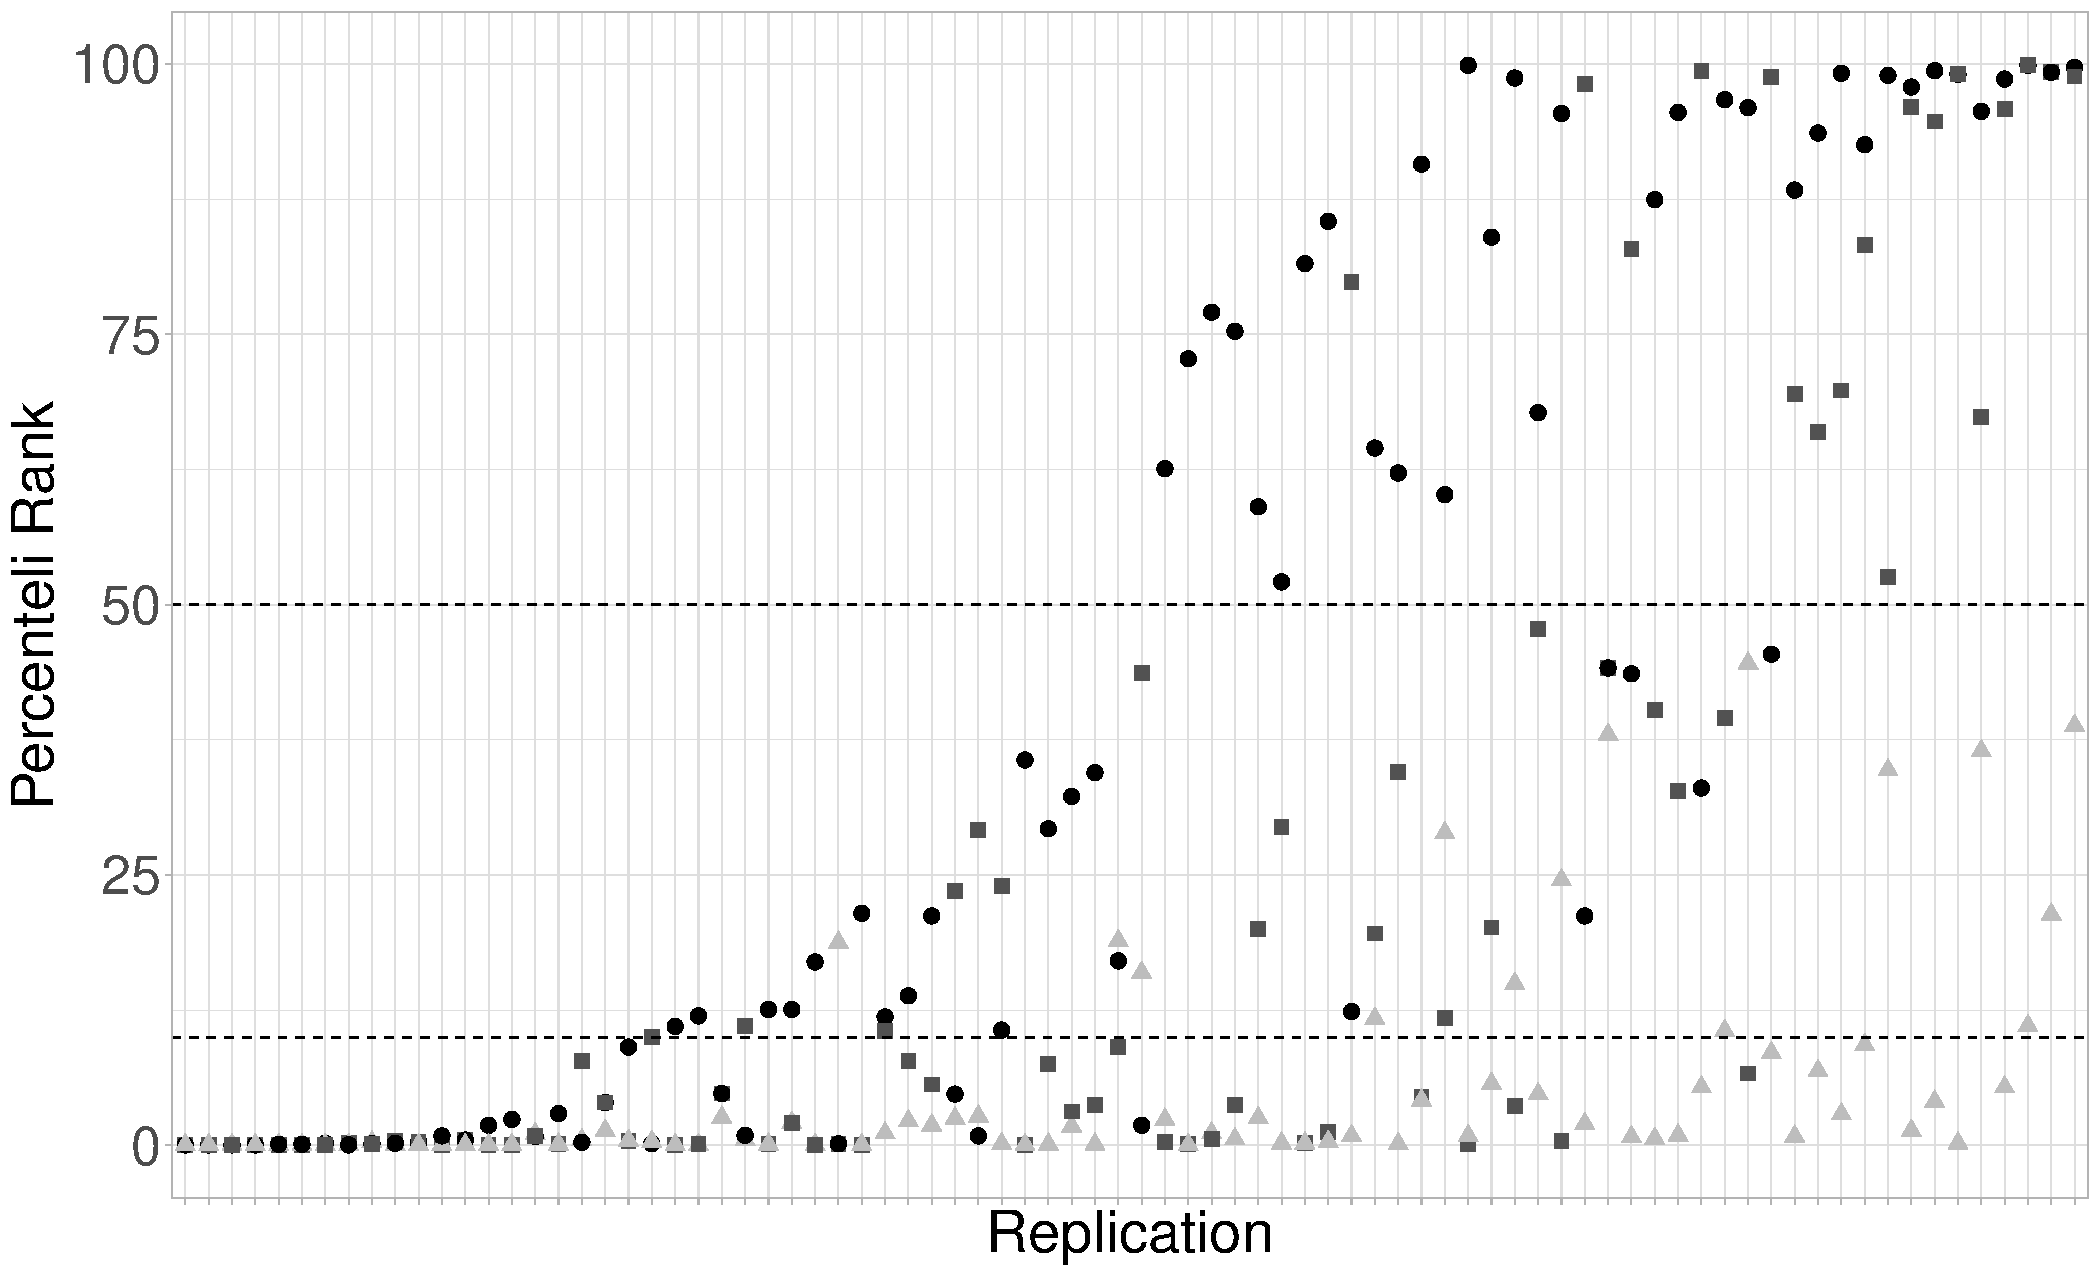
\includegraphics[width=\linewidth]{img/precentile-rank}
	\caption{Percentile ranks of the distances from the STFs chosen by Bruto and the STFs produced by ILA (square), ISA (dot), and Frank (triangle). The horizontal dashed lines represent the 10\textsuperscript{th} and 50\textsuperscript{th} percentiles.}
	\label{fig:percentile-rank}
\end{figure}
All the STFs developed by Frank were within the 50 percentile of distance, while the STFs developed by ILA and ISA exceeded the 50 percentile in the 22\% and 42\% of cases. 
Frank resulted in STFs over the 10 percentile of distance in the 18\% of cases, ILA and ISA in the 44\% and 67\% of cases, respectively.


The average symmetric distances from Bruto were:  $Q_{\text{ILA}}\Delta Q_{\text{Bruto}} = 2.70$, $Q_{\text{ISA}}\Delta Q_{\text{Bruto}} = 2.87$ and $Q_{\text{Frank}} \Delta Q_{\text{Bruto}}= 2.46$. The item selections of all the algorithms, on average, presented at least 2 items of difference from the selection provided by Bruto, with ISA showing the worst performance and Frank the best one. However, by only considering the symmetric distance it is not possible to ascertain whether these results were mostly ascribable to an over selection of items not included in bruto (lack of sensitivity) or an under selction of items included in Bruto (lack of sensitivity).
To better understand the results on the symmetric distance, 
Table \ref{tab:accuracy} reports the mean accuracy, sensitivity (i.e., items selected by Bruto and $x$), and specificity (i.e., items selected by neither Bruto nor $x$). 



 

\begin{table}[!h]
	\centering
	\caption{\label{tab:accuracy} Accuracy, sensitivity and specificity of the algorithms with respect to the best selection provided by Bruto.}
	\begin{tabular}{l c c c}
		\hline
		Algorithm	&	Accuracy	&	Specificity	&	Sensitivity	\\\hline
		ILA	&	0.56 $\pm$ 0.33	&	0.68 $\pm$ 0.39	&	0.43 $\pm$ 0.36	\\
		ISA	&	0.54 $\pm$ 0.32	&	0.64 $\pm$ 0.38	&	0.41 $\pm$ 0.37	\\
		Frank	&	0.59 $\pm$ 0.34	&	0.68 $\pm$ 0.38	&	0.50 $\pm$ 0.37	\\\hline
		
	\end{tabular}
\end{table}


Across the 82 replications, Frank provided the highest average accuracy, followed by ILA and ISA. It is worth noting that the accuracy of all algorithms was below the 60\%. 
The McNemar test suggested that, when compared against Bruto, Frank performed better than both ILA and ISA ($\chi^2 = 4.90$ and $\chi^2 = 10.58$, respectively), while no significant differences were found between ISA and ILA ($\chi^2 = 2.43$).
To best understand the implications of the results on the accuracy of the algorithms (i.e., whether they are mostly due to an over inclusion of items or an over exclusion of items), the average specificity and sensitivity should be considered. Frank and ILA resulted in the same average specificity, while the sensitivity of ILA was lower than that of Frank. In other words, Frank and ILA, on average, had the same ability of not selecting the items for inclusion in the STF as Bruto. However, ILA was less able than Frank in selecting for the inclusion in the STF the same items as Bruto. The lower accuracy of ILA compared to Frank is hence mostly due to ILA's inability of selecting for inclusion the same items as Bruto. 
ISA showed the least accuracy and specificity of all the algorithms, although its sensitivity was in line with that of ILA. 

\section*{Final Remarks}

This manuscript presented new IRT-based algorithms for the development of STFs. The functioning of the algorithms depends on the specification of the desired characteristics through the definition of a target information function.
While all algorithms aim at reducing as much as possible the distance between the provisional information function of the STF and the target information function, they differentiate according to the methods employed for considering the items for inclusion in the STF at each iteration. Specifically, two algorithms (ILA and ISA) consider either the location or the informativeness of the items in the full-length test with respect to specific latent trait levels, while the third one (Frank) considers the ability of each item in the full-length test of getting the provisional and target information functions closer. 

The results of a simulation study where the performance of the algorithms has been compared against that of a brute force algorithm showed that Frank was the only one (besides the brute force one) to always retrieve a STF. Moreover, Frank is the algorithm best able to recreate the TIF-target and to get as close as possible to the item combination selected by the brute force algorithm.

Even among the replications where all the algorithms identified a STF, Frank tended to identify the item selection that was closest, in terms of average distance, from that identified by the brute force algorithm. This result is not surprising given that Frank considers the contribution of each item in reducing the distance from the TIF-target across the entire latent trait rather than focusing on a specific level. By focusing on a specific level of the latent trait, like ILA and ISA do, and selecting the item that only helps in reducing the distance from the TIF-target for that level, the risk is that even items that are not close to the level, and hence do not help in bridging the gap from the TIF-target, can be selected for the evaluation. As such, not useful items (i.e., items that do not reduce the distance) might be included, leading to the termination criterion. On the other hand, Frank considers for the inclusion the item that contributes to reduce the distance from the TIF-target across all levels of the latent trait.


%Given that the TIF is an additive function of the IIFs, it increases as the number of  items in the test increases. For this reason, the mean TIF was considered. 
The TIF of a STF would always be lower than the TIF that could be obtained from the full-length test, meaning that generally a STF is less precise than the full-length test in measuring the latent trait. 
The true advantage of using a STF lies in the fact that respondents would get less tired, and their response accuracy should be maintained during the administration. This may be particularly useful when multiple tests are administered to reduce the overall cognitive burden on the respondents.   
This point should be further investigated in future simulation and empirical studies, where the tiredness of the respondents during the administration is accounted for by the algorithm for each administered item.

 
%All algorithms share the same aim (i.e., reducing the distance from a target information function that describes the desired characteristics of a test) and the same termination criterion, but they differ according to the methods used for considering the items for inclusion  in the STF. 
%All algorithms aim at minimizing the distance from a predefined TIF-target that describes the desired characteristics of the STF. 
%They differ according to the method used for the selection of the item for inclusion in the STF.  
%Two algorithms ground the item selection on the ability of each item of reducing the distance from the TIF-target with respect to a single discrete $\theta$ value, denoted as $\theta_{\text{target}}$. In one case (i.e., item locating algorithm, ILA), the item whose location is the closest to the $\theta_{\text{target}}$ is included, while in other case (i.e., item selecting algorithm, ISA) the item that is most informative with respect to the $\theta_{\text{target}}$ is selected.
%Another algorithm (i.e., Frank) considers the ability of each item of reducing the distance from the TIF-target with respect to the entire latent trait. 
%Besides of the aim, the algorithms share the termination criterion. Specifically, at each iteration an item (i.e., provisional item) is selected from the full-length test according to the algorithm-specific method and is considered for the inclusion in the STF.
%\alert{Non sono sicura della posizioen della spiegazione del criterio di terminazione}
%The termination criterion tests whether other items should be added in the STF by considering the distance between the TIF-target, the TIF obtained by including the provisional item, and the TIF obtained by excluding the provisional item. If the distance between the former two is greater than or equal to the distance between the latter two, the provisional item is not included in the STF and the algorithm stops. Vice versa, the item is included and the algorithms proceeds to a new iteration. The reasoning is as follows. If the distance from the TIF-target of the STF including the provisional item is greater than or equal to the difference from the TIF-target of the STF without the provisional item, it means that the provisional item does not contribute in reducing this distance. Since the provisional item is the best one among the available options according to the selection method of each algorithm, but does not contribute to reduce the distance from the TIF-target, the algorithm stops, assuming that no further useful items remain.


%Gonzalez forme breve IRT ML accuartezza forme bevi proprio nel prevedere una diagnosi.
\newpage
\bibliographystyle{apacite} 
\doublespacing
\bibliography{bibFile}

\end{document}
